\documentclass[a4paper,openany,12pt]{book}
%%%%%%%%%%%%%%%%%%%%%%%%%%%%%%%%
%%%% DEFINICIÓN DE PAQUETES %%%%
%%%%%%%%%%%%%%%%%%%%%%%%%%%%%%%%
\usepackage{tocloft}
\usepackage[utf8]{inputenc}
\usepackage{CJKutf8}
\usepackage[spanish]{babel}
\usepackage{fancyhdr}
\usepackage{ragged2e}
\usepackage{setspace}
\usepackage{cite}
\usepackage{enumerate}
\usepackage[font={color=RBlue},figurename=Fig.]{caption}
\usepackage{graphicx}
\usepackage{subfigure}
\usepackage{hyperref}
\usepackage{eurosym}
\usepackage{pdfpages}
\usepackage{multirow, array}
\usepackage{float}
\usepackage{longtable}
\usepackage{xcolor,colortbl} 
%Paquete para crear colores específicos según RGB.
\usepackage{geometry}
%Paquete para definir las dimensiones de los márgenes.
\usepackage{lscape}
\usepackage{rotating}
\usepackage{amsmath}
\usepackage{multicol}
\usepackage[nottoc,notlot,notlof]{tocbibind}
\usepackage[titletoc]{appendix}
\usepackage{notoccite}
\usepackage{acronym}
\usepackage[colorinlistoftodos]{todonotes}
% added packages
\usepackage{listings}
\usepackage{enumitem}% http://ctan.org/pkg/enumitem



\newenvironment{Figure}
  {\par\medskip\noindent\minipage{\linewidth}}
  {\endminipage\par\medskip}
\setlength{\columnsep}{1cm}
\DeclareUnicodeCharacter{2061}{}

\definecolor{RBlue}{RGB}{23,33,110} 
\definecolor{Rojo}{RGB}{255,0,0}
\definecolor{Cyan}{RGB}{214,234,240}
\definecolor{Naranja}{RGB}{255,222,199}
\definecolor{GrisTabla}{RGB}{245,245,245}
%Ejemplo de funciones para definir colores a utilizar el documento, según sus dígitos RGB.


%%%%%%%%%%%%%%%%%%%%%%%%%%%%%%%%%%%%%%%%%%%%%%%%%%%%%%%%%%%
%%%% PROPIEDADES DEL DOCUMENTO (Funciones específicas) %%%%
%%%%%%%%%%%%%%%%%%%%%%%%%%%%%%%%%%%%%%%%%%%%%%%%%%%%%%%%%%%

%\setcounter{secnumdepth}{3} 
%Esta función permite que en el índice se indique hasta el sub-nivel número tres. Es decir que aparezcan hasta los apartados 1.1.1. Si se indicase {4}, se podrían observar hasta los sub-apartados 1.1.1.1. 

%\setlength{\headsep}{0.5in} 


\onehalfspace 

\setlength{\parskip}{1em}
\setlength{\parindent}{0cm}

\includeonly{
    Chapter/intro,
    Chapter/01_antecedentes,
    Chapter/02_objalc,
    Chapter/03_desarrollo,
    Chapter/04_planificacion,
    Chapter/05_cargas,
    Chapter/06_presupuesto,
    Chapter/07_conclusiones,
    Chapter/08_valoracion,
    Chapter/10_biblio,
    Chapter/00_requisitos,
    Chapter/000_repo,
    Chapter/09_anexo,
}
%Esta función es de gran importancia. Como se puede observar a la izquierda, hay una carpeta que se ha creado con diferentes capítulos. Estos capítulos son los diferentes apartados de la memoria en los que se va a ir escribiendo. Por ejemplo, el capítulo de la introducción, el capítulo de objetivos, el capítulo de la memoria técnica, o el capítulo del plan de trabajo. Bien, de cara a poder incluirlos a posteriori en esto documento principal (MAIN.tex) es necesario indicarle a LATEX que los cargue y eso se realiza con esta función. Así, habrá que incluir tantos parámetros como capítulos se deseen cargar. Los parámetros son simplemente la dirección de la carpeta en la que se encuentran, y su nombre.

\geometry{top=3.5cm, bottom=2.5cm, left=2.5cm, right=2.5cm}
%Esta función determina los márgenes que se han de utilizar a lo largo de todo el documento. Así, el margen superior será de 3.5 y el resto de 2.5 cm .


%%%%%%%%%%%%%%%%%%%%%%%%%%%%%%%%%%%%%%%%%%%%%%%%%%%%%%%%%%%%%%%%
%%%% COMIENZA EL DOCUMENTO (con la función \begin{document} %%%%
%%%%%%%%%%%%%%%%%%%%%%%%%%%%%%%%%%%%%%%%%%%%%%%%%%%%%%%%%%%%%%%%


\begin{document}

%%%%%%%%%%%%%%%%%%%%
%%%% PAGINACIÓN %%%%
%%%%%%%%%%%%%%%%%%%%

\pagestyle{fancy}
%Esta función es utilizada para crear un nuevo estilo de formato, es el formato "fancy". En él vamos a determinar a continuación cómo se quieren posicionar pies de página, encabezados y demás.

\lhead{}
%Esta función sirve para que no se escriba nada (parámetro obligatorio vacío) en el encabezado en la posición izquierda. 

\chead{}

\rhead{}

\cfoot{}

\fancyfoot[L]{\thepage} 

\renewcommand{\headrulewidth}{0pt} 


\includepdf[]{PDF/Por0}
\newpage

\includepdf[]{PDF/Por1}
\newpage
\frontmatter

\setcounter{page}{3}

%Esta función permite comenzar el contador de las páginas para la numeración en el número 3, es importante puesto que los primeros números van dedicados a portada y contraportada y no se numeran. Así, la primera página numerada será la 3. 
\section*{Resumen}
\thispagestyle{fancy}
\fancyhead[L]{PROYECTO DE FIN DE GRADO}
Este proyecto de fin de grado trata del diseño y desarrollo de una aplicación no nativa con la que podremos medir la cantidad de partículas en suspensión (PM2.5, o PM10)que se encuentran en el aire. 
Para este fin, la aplicación hace uso de procesamiento de imágenes.
En primer lugar, contamos con una página web que es la encargada de mostrar los datos de la contaminación que hemos obtenido mediante la carga y procesamiento de imágenes.
En segundo lugar, disponemos de un Bot que puede recibir imágenes, que el usuario habrá tomado, estas imágenes se analizaran y se devuelven los resultados de la contaminación detectada en la fotografía.
De la fotografía nos interesa su ubicación para poder geo posicionarla. Una vez que el análisis de la imagen  haya sido efectuado obtendremos los datos de la contaminación en el aire. Estos datos serán almacenados en una base de datos y posteriormente cargamos estos datos en nuestra página web. 
Una vez la carga haya sido efectuada con éxito, podremos visualizar los datos con facilidad en una web cuyo objetivo será permitirnos ver de forma amigable la contaminación detectada en el aire en ciertas zonas.
\section*{Descriptores}
PM2.5,PM10,Bot, Web,Telegram
\clearpage
\fancypagestyle{plain}{}
%Se define mediante esta función el formato plain, que no tiene nada, ni encabezados ni pies de página. Realmente esta función podría ir a comienzo del documento o en cualquier lugar, es decir, se puede mover.

\tableofcontents
%Esta función permite introducir el índice de capítulos (hasta el subíndice que se haya indicado previamente).
\newpage
\listoftables
%Por ultimo, se introduce el índice de tablas en caso de que las hubiera en vuestro documento. 
\mainmatter
%Esta función se utiliza para indicar que a partir de ahora la numeración pasa a ser con números estándar y no con romanos como se había venido utilizando hasta ahora.

\pagestyle{fancy}
%A continuación se vuelve a redefinir el estilo “fancy” para que se adecúe al que ha de utilizarse a lo largo de toda la memoria. El estilo es el siguiente:

\lhead{}


\chead{}


\fancyhead[OL]{PROYECTO FIN DE GRADO}
%En el encabezado a la derecha en las páginas pares se escribe: "PROYECTO FIN DE GRADO".

\fancyhead[OL]{PROYECTO DE FIN DE GRADO} 


\fancyhead[L]{}


\cfoot{} 


\fancyfoot[L]{\thepage} 


\renewcommand{\headrulewidth}{0pt} 
\bibliographystyle{IEEEtran}
\chapter{Introducción}\label{Int}
\fancyhf{}% Clear header/footer
\fancyhead[L]{INTRODUCCIÓN}
\fancyfoot[L]{\thepage} 
\section{Introducción}
En el presente documento se recoge una definición detallada del proyecto, así como los antecedentes y su justificación, el desarrollo, la planificación llevada a cabo para su realización, junto con el presupuesto empleado y finalmente las conclusiones y los
resultados obtenidos tras el proyecto. El documento se desglosa en los siguientes capítulos:
\begin{itemize}
    \item \textbf{Introducción: }
    Presentación de los contenidos del proyecto y de la estructura de
apartados.
    \item \textbf{Antecedentes y Justificación: }
    Una descripción del entorno del proyecto y del estado del arte actual en cuanto a aspectos técnicos, económicos y sociales, junto con una justificación técnica de la ejecución y viabilidad del proyecto.
    \item \textbf{Objetivos y Alcance: }
    Establecimiento del objetivo principal del proyecto, así como su alcance. Se nombran los aspectos funcionales que incluye y los que excluye. Estos objetivos han estado muy presentes a lo largo de todo el proyecto, desde las primeras fases de diseño hasta las últimas etapas de desarrollo.
    \item\textbf{Requisitos: }
    Identificación de los requisitos del proyecto.
    \item \textbf{Desarrollo: }
    En este apartado se describe el desarrollo, para implementar eficazmente el software, a presentar como proyecto final de grado.
    \item \textbf{ Planificación: }
    Descripción detallada del equipo de trabajo, enumeración y
especificación de las actividades realizadas junto con los tiempos de realización, un
diagrama de Gantt que recoge el tiempo y la dedicación de las tareas a lo largo del
diseño y desarrollo del sistema.
    \item\textbf{Cargas de trabajo: }
    Exposicion de las cargas de trabajo enfrentadas a la hora de elaborar el proyecto 
    \item\textbf{Presupuesto:}
    Descripción de los gastos que supondría elaborar este proyecto si se fuera a contratar a gente para desarrollarlo, así como los gastos en software.
    
    \item \textbf{ Conclusiones: }
    Conclusiones obtenidas al final el proyecto, así como posibles mejoras.
    \item\textbf{Valoración:}
Capítulo final donde, una vez finalizado el proyecto, se procede a tomar y exponer las
conclusiones del mismo. En esta parte también se han expuesto los resultados del producto final, así como una valoración personal y otra valoración ética.
\item\textbf{Repositorio Github}:
Enlace al respositorio de Github

\item\textbf{Anexo:}
Explicacion de las tecnologias usadas asi como un manual de uso
    
\end{itemize}
\chapter{Antecedentes y justificación}\label{Int}
\fancyhf{}% Clear header/footer
\fancyhead[L]{PROYECTO DE FIN DE GRADO}
\fancyfoot[L]{\thepage} 
%\section{Antecedentes y Justificación}

\section{Antecedentes y estado del arte}

La contaminación atmosférica es un problema generalizado que afecta tanto a la salud humana como al medio ambiente. Para adoptar medidas preventivas, es crucial detectar a tiempo la contaminación atmosférica. Sin embargo, la medición actual de la contaminación atmosférica se basa en estaciones de control caras y poco accesibles. El objetivo de mi proyecto es ofrecer una solución práctica y asequible al problema de la detección de la contaminación atmosférica utilizando imágenes captadas por el usuario. Algún ejemplo de esto serían
los siguientes:
\begin{itemize}
    \item Análisis de laboratorio de muestras de aire: Este proceso es costoso y requiere tiempo y esfuerzo para recopilar y enviar muestras a un laboratorio.
    \item Sistemas de monitoreo de redes:  Estos sistemas requieren la instalación de sensores en varios puntos de la ciudad y suelen ser costosos y difíciles de acceder para la mayoría de la población.
    \item Tecnologías de satélite: Este enfoque es costoso debido a la necesidad de desarrollar y lanzar satélites especializados.
\end{itemize}
A nivel estatal, los niveles de PM10 siempre han sido altos, esto en parte es se debe a las incursiones de masa de aire africano proveniente del desierto del Sahara. En 2021 se empezó a modelar y estimar la cantidad de partículas provenientes de las masas de aire Africanas y se observó que 9 de cada 10 estaciones exceden sus niveles de VLD y VLD en las mediciones que se tomaron.
Teniendo en cuenta estos aspectos, podemos deducir que respiramos aire de dudosa calida, ademas, el numero de estaciones fijas por habitante a nivel estatal es escaso,atendiendo a la informacion que arrojan estas estaciones es importante destacar que existen zonas que superan frecuentemente el nivel maximo de exposicion diaria y anual a PM10 recomendado por la OMS\\
Existen varios índices para medir la contaminación en el aire, pero para este proyecto nos centraremos en los índices basados en partículas en suspensión en el aire, más concretamente las denominadas como PM10  y PM2.5 por sus siglas (Partículas menores xx a micrómetros).
Empezaré exponiendo por que es importante tener en cuenta estas partículas para la detección del estado de calidad del aire:
Estas partículas tienen un tamaño significativamente pequeño, su diámetro varia entre 2,5 y 10 micrómetros, para que el lector de este documento pueda imaginar claramente su tamaño aclararemos que 1 micrómetro corresponde a una milésima parte de un milímetro.
Las PM10 son capaces de penetrar has las vías respiratorias bajas.
Seguido, nombraré algunas enfermedades que pueden ser generadas por cuando respiramos aire, que contiene niveles perjudiciales para la salud de PM10 y PM2.5:\\

\begin{itemize}
    \item Tos o dificultad para respirar
    \item infartos de miocardio
    \item Asma
    \item Cáncer de pulmón
\end{itemize}
En cuanto a las PM2.5 estas partículas son capaces de penetrar hasta las zonas de intercambio de gases del pulmón.El origen de estas partículas proviene  mayoritariamente de las emisiones de vehículos.
Estas partículas no solo son las culpables de efectos adversos en la salud humana tambien tienen efectos adversos sobre el medio ambiente ya que estas partículas son movidas por el viento y son capaces de instalarse en el suelo o en el agua causando daños medio ambientales como los siguientes:\\
\begin{itemize}
    \item Acidificación de los lagos y arroyos
    \item Reducción de los nutrientes del suelo
    \item Efectos perjudiciales sobre la diversidad de ecosistemas
    \item Contribución a los efectos de lluvia ácida
\end{itemize}




Actualmente, existen soluciones costosas y poco accesibles para detectar la contaminación del aire. Sin embargo, la tecnología de procesamiento de imágenes ha avanzado significativamente en los últimos años y es posible desarrollar una solución económica y accesible para detectar la contaminación del aire a través de imágenes capturadas por los usuarios. Este proyecto se diferencia de las tecnologías nombradas anteriormente, ya que proporciona una solución accesible y asequible que utiliza tecnologías existentes, como puede ser el uso de :
\begin{itemize}
    \item  Bot de Telegram.
    \item Cámaras móviles.
    \item API de Google maps.
\end{itemize}

Además, al permitir a los usuarios contribuir con datos sobre la calidad del aire, este proyecto también aborda la necesidad de una mayor participación ciudadana en la monitorización de la calidad del aire.
Esto fomenta la denominada ciencia ciudadana,El libro blanco para la ciencia ciudadana para Europa define la ciencia ciudadana con el siguiente termino:\\
"La participación de la ciudadanía en actividades de investigación científica en la que los ciudadanos contribuyen activamente a la ciencia con su esfuerzo intelectual, sus conocimientos o con sus herramientas y recursos."\\
En la misma línea, en abril de 2020, la Asociación Europea de Ciencia Ciudadana publicó las principales características de su enfoque de CC (Haklay, 2020). Este gran ejercicio está estrechamente relacionado con los diez principios de la Ciencia Ciudadana también definidos por la misma asociación que se listan a continuación.
\begin{enumerate}
    \item Los proyectos de ciencia ciudadana involucran activamente a los y las ciudadanas en tareas
científicas que generan nuevo conocimiento o una mejor comprensión.
    \item Los proyectos de ciencia ciudadana producen un resultado científico nuevo
    \item Tanto los y las científicas profesionales como los y las científicas ciudadanas se benefician de
la participación
    \item Los y las científicas ciudadanas pueden, si lo desean, participar en múltiples etapas del proceso
 científico 
    \item Los y las científicas ciudadanas deben recibir información del proyecto en todo momento
    \item La ciencia ciudadana representa un tipo de investigación como cualquier otro, con sus
limitaciones y sesgos que hay que considerar y controlar
    \item Los datos y meta-datos de proyectos de ciencia ciudadana deberían ser públicos y a ser posible,
los resultados deberían publicarse en un formato de acceso abierto
    \item Los y las científicas ciudadanas deben estar reconocidos en los resultados y publicaciones del
proyecto
    \item Los programas de ciencia ciudadana deben evaluarse por su producción científica, la calidad de
los datos, la experiencia de los y las participantes y el alcance del impacto social o político
    \item Los líderes de proyectos de ciencia ciudadana deben tener en cuenta tanto los aspectos legales
y éticos como los derechos de autor, la propiedad intelectual, los acuerdos de intercambio de
datos, la confidencialidad, la atribución y el impacto ambiental de sus actividades
    
\end{enumerate}
La ciencia ciudadana está cobrando un papel cada vez más importante en la investigación. Cabe resaltar que en la Estrategia Española de Ciencia, Tecnología e Innovación 2021-2027 (EECTI) (España, 2020, p. 34), la CC aparece explícitamente como herramienta para fomentar uno de los principios de la EECTI: La responsabilidad social y económica en la I+D+I y la aplicación de la co-creación y las políticas de acceso abierto, así como, el alineamiento de la I+D+I con los valores, necesidades y expectativas sociales. La educación reglada a nivel estatal no es mera espectadora del avance científico y es por ello por lo que el anteproyecto de Ley Orgánica del Sistema Universitario e habla del rol de la CC para el fomento de la ciencia abierta. De forma específica, en el artículo 15: Cohesión social y territorial se indica: <<Las universidades promoverán un desarrollo económico y social equitativo, inclusivo y sostenible, [..] A tal efecto, reforzarán la colaboración con las Administraciones Locales y con los actores sociales de su entorno mediante los proyectos de Ciencia Ciudadana [..]>>. Además, se refiere completamente al fomento de la Ciencia Ciudadana y la Ciencia Abierta que inspira esta práctica:

\textbf{Se fomentará la Ciencia Ciudadana como un campo de generación de conocimiento compartido entre la ciudadanía y el sistema universitario de investigación. Por último, la norma busca ahondar y asegurar una Universidad autónoma, democrática y participativa que constituya un espacio de libertad, de debate cultural y de desarrollo personal al mismo tiempo que sea eficaz y eficiente en la toma de decisiones y su gestión el artículo (Artículo 63, apartado 10).}

A nivel de participación, según la literatura consultada, existen varias tipologías de proyecto de ciencia ciudadana dependiendo del grado en el que se incorpore o involucre la ciudadanía en el proceso científico. La "inteligencia distribuida" (Howe, 2006), "Ciencia participativa" (Bonney et al., 2009) y "Ciencia Ciudadana Extrema" (ECS, por sus siglas en inglés) (Haklay, 2013). Esta última categoría busca específicamente poner las herramientas y métodos científicos al alcance de cualquiera. Es decir, la ECS propone que todas las personas, independientemente de su nivel de alfabetización o conocimientos previos, puedan involucrarse de todo el proceso científico, desde la definición de los problemas de su entorno o que les atañen y la colaboración en la recogida de datos, hasta el uso de los resultados para abordar y resolver los problemas identificados por las propias comunidades. En la misma línea, los proyectos de investigación colectivos se clasifican en una escalera de participación, en cada peldaño que se sube la colaboración es mayor en todos los ámbitos de la ciencia (Arnstein, 1969). De esta forma, y análogamente a la taxonomía previa, existen proyectos contributivos (principalmente la ciudadanía colabora recogiendo y recopilación datos para que otras personas o entidades los usen); proyectos colaborativos (donde la ciudadanía participa de la recopilación de datos y perfeccionamiento del diseño del proyecto, en el análisis de datos y en la difusión de resultados); y finalmente en proyectos cocreados o co-creativos (que son diseñados conjuntamente por científicos y ciudadanía en los que el público de a pie comparte la responsabilidad de la mayoría o de todos los pasos de un proyecto/proceso científico). Por último, se ha encontrado un trabajo de investigación (Aristeidou et al., 2017) que se centra en el nivel de participación de la ciudadanía teniendo en cuenta los rasgos de comportamiento y las necesidades personales encontrando cinco tipos de usuarios en la ciencia ciudadana: trabajadores, persistentes, leales, los que están al acecho y visitantes.


\section{Justificación}
La justificación técnica de este proyecto se basa en la necesidad de una solución asequible y práctica para la detección de la contaminación atmosférica. Actualmente, la mayoría de la población considera que muchas de las soluciones existentes son caras y de difícil acceso, lo que limita su capacidad para controlar y comprender la calidad del aire en sus comunidades.

Además, la contaminación del aire es un problema global que afecta la salud humana y el medio ambiente, por lo que es importante que se desarrollen soluciones accesibles y asequibles para monitorear y comprender su impacto. Al permitir a los usuarios contribuir con datos sobre la calidad del aire, nuestro proyecto también promueve la participación ciudadana en la monitorización de la calidad del aire.

Desde el punto de vista técnico, este proyecto es viable gracias a la disponibilidad de tecnologías como las cámaras de los teléfonos móviles y las API de Google Maps, que permiten recopilar y procesar información sobre la calidad del aire de forma fácil y asequible. Además, el uso de un bot de Telegram y un sitio web construido en Django permite integrar y visualizar los resultados de forma sencilla, lo que facilita a los usuarios la comprensión y el uso de los datos.

En conclusión, la justificación técnica de este proyecto se basa en la necesidad de una solución asequible y práctica para la detección de la contaminación atmosférica, así como involucrar a la ciudadanía en campañas de captación colectiva de datos de calidad del aire basadas en ciencia ciudadana y en la disponibilidad de tecnologías existentes que permiten su desarrollo y aplicación.
\chapter{Objetivos y alcance}\label{Int}
\fancyhf{}% Clear header/footer
\fancyhead[L]{PROYECTO DE FIN DE GRADO}
\fancyfoot[L]{\thepage} 
\thispagestyle{fancy}
\section{Objetivos}
El objetivo de este trabajo es el de Diseño y Desarrollo de una App móvil
multiplataforma que detecte contaminación atmosférica mediante fotografías, para esto haremos uso de un bot de Telegram y una web que nos mostrara el contenido de manera amigable.
\begin{itemize}
    \item El sistema ha de ser desacoplado para que este pueda ser fácilmente mantenible y escalable
    \item El sistema será fluido y con tiempos de respuesta aceptables
\end{itemize}
Se alcanzara el objetivo mediante una elección coherente de arquitectura, software y una buena programación del sistema
\section{Alcance}
Se trata del diseño y desarrollo de una app móvil multiplataforma capaz de detectar la contaminación atmosférica mediante fotografías.
Para poder lograr esto haremos uso de un bot de Telegram en el que el usuario subirá la imagen en la que se han quedado las partículas y también mandara la ubicación en donde la imagen fue tomada.
Una vez el bot tenga la imagen y la ubicación la imagen será procesada para contar las partículas en ella, con esta información se mandara una petición HTTP  de tipo post a la base de datos de la web y alojara la información para posteriormente mostrarla en el mapa.
A continuación, se define brevemente el alcance de cada una de las partes implicadas en el sistema.
En conclusión, el sistema ha de reflejar la estructura mencionada con base en un desarrollo software coherente. Queda fuera del alcance del sistema la aplicación de técnicas de inteligencia artificial para procesar las imágenes, así como para reconocer el tipo de imagen, o forzar al usuario a meter una imagen especifica, es decir, se dará por hecho que el usuario siempre meterá una imagen correcta. También quedan fuera  temas relacionados con ciberseguridad a la hora de mandar la información a la base de datos, esta parte ha quedado fuera, ya que el proyecto se desarrolla en la una máquina local  y solo yo tengo acceso a esta información. Siendo mejoras que se podrían llevar a cabo en futuras ampliaciones del proyecto o en un despliegue final.
A continuación, se define brevemente el alcance de cada una de las partes implicadas en el
sistema.

\subsection{Bot de Telegram}
El bot se encarga de recibir la información relevante, a la ubicación y la imagen. Esta parte implica la creación del bot y el uso de las API oficiales de Telegram y el desarrollo del código referente a la puesta en marcha del bot.
\subsection{Web}
La página web nos sirve para visualizar de una manera amigable la información que ha sido cargada previamente por otros usuarios y está alojada en una base de datos propia de Django.
\subsection{Procesamiento de la imagen:}
Se usa una función llamada suavizar incluida en el bot de Telegram para procesar la imagen subida por el usuario, esta función tiene como objetivo procesar una imagen específica para suavizarla y resaltar las manchas presentes en ella.

\chapter{Requisitos}\label{Int}
\fancyhf{}% Clear header/footer
\fancyhead[L]{PROYECTO DE FIN DE GRADO}
\fancyfoot[L]{\thepage} 
Es importante identificar los requisitos funcionales y no funcionales en un proyecto informático porque esto asegura que el sistema desarrollado cumpla con las expectativas y necesidades del cliente o usuario final.
\section{Funcionales}Requisitos funcionales:
Los requisitos funcionales describen qué debe hacer el sistema.
a continuación listaré los referentes a este proyecto.
\begin{enumerate}
    \item El bot de Telegram debe permitir que el usuario suba una foto y su ubicación
    \item La función de tratamiento de imágenes debe detectar el número de puntos en la imagen
    \item La aplicación web de Django debe mostrar la ubicación de la foto y el nivel de contaminación en un mapa
\end{enumerate}


\section{No funcionales}
Los requisitos no funcionales son aquellos que describen cómo debe ser el sistema en términos de características de calidad, como rendimiento, escalabilidad, usabilidad, entre otros.
\begin{enumerate}
    \item La aplicación debe ser fácil de usar e intuitiva
    \item La aplicación debe tener un tiempo de respuesta rápido y eficiente en términos de recursos
    \item La aplicación debe ser escalable para manejar una alta cantidad de usuarios y datos
\end{enumerate}


\chapter{Desarrollo}\label{int}
\thispagestyle{fancy}

\section{Fase Inicial}
Una vez definido el objetivo del proyecto pasaremos a diferencias las partes más relevantes que se desean implementar.
\begin{itemize}
    \item Bot de Telegram
    \item Algoritmo para procesar imágenes
    \item Página web
\end{itemize}
Tras enumerar todos los componentes del sistema, es necesario definir su estructura de diseño. El término "arquitectura de software" se refiere al proceso de definir los numerosos componentes que conforman un sistema y cómo se comunican entre sí utilizando un conjunto de directrices y abstracciones. En este caso, se ha optado por una arquitectura de microservicios, que se describe a continuación.
\section{Arquitectura}

La arquitectura de la aplicación está diseñada para gestionar el procesamiento y análisis de imágenes de partículas y su localización. Consta de tres componentes clave: el bot de Telegram, el módulo de procesamiento de imágenes y la interfaz web.

El bot de Telegram, codificado en Python, permite a los usuarios cargar una imagen de partículas y su ubicación. La imagen es examinada por el módulo de procesamiento de imágenes, que también determina dónde se encuentran las partículas. Este módulo se construye con Python y varias bibliotecas de procesamiento de imágenes, como OpenCV.

La interfaz web se encarga de mostrar los resultados del procesamiento de imágenes y la localización de partículas. 

Toda la arquitectura está diseñada para ser modular y fácilmente ampliable, de modo que en el futuro puedan añadirse nuevos algoritmos o funciones de procesamiento de imágenes. Además, el sistema está diseñado para ser escalable.

Para nuestro caso en particular se identifican los siguientes servicios:
\begin{itemize}
    \item \textbf{Bot de Telegram}:
    Se encargará de la interacción a través de Telegram con el usuario, para esto el usuario mandará unos datos al bot y una vez recolectados y procesados estos datos serán mandados a la web.
    \item\textbf{ Procesamiento de imagen:}
    Una vez el usuario ha subido la foto, se procesará la imagen usando ciertos filtros y conversión de la imagen a escala de grises para obtener el resultado.
    \item \textbf{Página web:}
    La utilizaremos para mostrar los resultados obtenidos, así como la ubicación donde se tomó la foto.
\end{itemize}
%\section{Diagrama de flujo}
\section{Bot de Telegram}
Se comenzó el desarrollo por la parte de la creación del bot de Telegram, ya que será el elemento con el cual el usuario entrara en contacto por primera vez y el que dará a pie a poder usar todo el sistema de la manera correcta. Además, al ser algo nuevo que podría requerir más tiempo, se vio acertado empezar por este apartado, ya que la creación de los otros elementos se tenía experiencia previa gracias a la formación académica recibida a lo largo de la carrera.

El proceso de desarrollo incluye la lectura de tutoriales y documentación oficial de Telegram sobre cómo crear bots en Telegram.
El primer paso es crear un bot en Telegram, para lo que es necesario instalar la aplicación de mensajería, ya que es así como se lleva a cabo el proceso. Telegram cuenta con un bot oficial que los desarrolladores pueden utilizar para crear bots y actualizar sus datos.

El contacto con el bot oficial de Telegram @BotFather se establece a través de una ventana de chat privada. El bot proporciona una lista de comandos que se pueden utilizar para crear y gestionar bots.
En esa lista de comandos se encuentra el comando /newbot, que permite crear un nuevo bot. Este es el primer comando que se utiliza. A continuación, el bot oficial solicita un nombre de usuario para crear el nuevo bot, que debe ser distinto de cualquier otro bot ya existente.

Una vez creado el bot, BotFather de Telegram proporciona el ID público del bot, que cualquier usuario puede utilizar para iniciar una conversación. Además, proporciona el token necesario para utilizar la API de bots de Telegram. De esta forma, se tiene acceso a todos los métodos de Telegram disponibles para conocer el funcionamiento del nuevo bot, incluyendo la capacidad de leer y enviar mensajes cuando un usuario contacta con él y un amplio abanico de otras capacidades.

Es crucial tener en cuenta que el token proporciona acceso completo al bot desarrollado; como resultado, por razones de seguridad, se debe tener cuidado de no revelar el token a terceros. En caso de filtración, se puede revocar el token actual utilizando el comando /revoke antes de generar uno nuevo.

\section{Instanciación y definición del bot}


Para instanciar el bot se utiliza el módulo Telegram y su extensión ApplicationBuilder. En primer lugar, se crea una instancia de ApplicationBuilder, a la que se le pasa el token del bot obtenido al crear el bot en Telegram.
El bot tiene como función procesar imágenes recibidas por el usuario y enviar los datos de la imagen procesada a una API. 
\subsection{Interacción con el usuario}
Cuando el usuario envía una imagen al bot, se utiliza la función suavizar para suavizar la imagen y contar los puntos detectados en ella. Luego, se envían los datos de la imagen procesada, como la contaminación detectada y la ubicación de la imagen, a una API mediante una solicitud HTTP POST. El bot también tiene la capacidad de recibir la latitud y longitud del usuario y guardar esta información para enviarla junto con los datos de la imagen procesada a la API. Utiliza también la librería "logging" para registrar eventos y errores en un archivo de registro.
\section{Procesar la imagen}
La función usa la biblioteca OpenCV para realizar las operaciones de procesamiento de imágenes, la función se llama tratar y recibe como argumentos una cadena de texto
\begin{enumerate}
    \item Carga una imagen utilizando la ruta especificada en el argumento 
    \item Verifica si la imagen se ha cargado correctamente y si no es así, lanza un error
    \item Aplica un filtro de diferencia de mediana a la imagen original
    \item Convierte la imagen suavizada a escala de grises
    \item Calcula la diferencia entre la imagen original y la imagen suavizada con el filtro de mediana
    \item Vuelve a convertir la imagen de diferencia a escala de grises
    \item Aplica el algoritmo Canny para detectar los bordes en la imagen en escala de grises
    \item Encuentra los contornos en la imagen usando Canny
    \item Verifica si se encontraron al menos un contorno y si no es así, lanza un error
    \item Dibuja los contornos encontrados en la imagen original y los marca en rojo
    \item Guarda la imagen con los contornos marcados en rojo
    \item Imprime el número de contornos encontrados 
    \item Calcula y devuelve el resultado, que es la cantidad de contornos dividido por 36
\end{enumerate}
\clearpage
\lstset{language=Python, breaklines=true, basicstyle=\footnotesize}
\begin{lstlisting}[frame=single]
def tratar(nombre_imagen): 
    # Cargar imagen y verificar que la ruta de la imagen es válida 
    img = cv2.imread(nombre_imagen) 
    # Verificar que la imagen se ha cargado correctamente 
    if img is None:
        raise ValueError("Nooooo se pudo cargar la imagen: ", nombre_imagen)
    # Aplicar filtro de diferencia de mediana 
    img_suave = cv2.medianBlur(img, 5) 
    # Convertir a escala de grises 
    img_gris = cv2.cvtColor(img_suave, cv2.COLOR_BGR2GRAY) 
    # Aplicar la diferencia entre la imagen original y la imagen suavizada con el filtro de mediana 
    img_diferencia = cv2.absdiff(img, img_suave) 
    img_gris = cv2.cvtColor(img_diferencia, cv2.COLOR_BGR2GRAY) 
    # Aplicar Canny para detectar los bordes
    img_canny = cv2.Canny(img_gris, 50, 150) 
    # Encontrar contornos 
    contornos, _ = cv2.findContours(img_canny, cv2.RETR_EXTERNAL, cv2.CHAIN_APPROX_SIMPLE) 
    # Verificar que se encontraron al menos un contorno 
    if len(contornos) == 0:
        raise ValueError("No se encontraron puntos en la imagen.") 
    # Dibujar los contornos encontrados en la imagen original en rojo 
    img_puntos = img.copy() 
    cv2.drawContours(img_puntos, contornos, -1, (0, 0, 255), 2) 
    # Guardar la imagen con los puntos detectados marcados en rojo 
    cv2.imwrite("imgpuntos.jpg", img_puntos) 
    # Imprimir el número de puntos encontrados 
    print("Número de puntos encontrados: ", len(contornos)) 
    result = len(contornos)/36 
    return result

\end{lstlisting}
\clearpage
\section{Interfaz web}
La interfaz web cumple con el objetivo de mostrar la información. Esta interfaz está construida con Django y tiene un front-end que utiliza JavaScript y HTML. La interfaz web también se comunica con una base de datos para almacenar las imágenes procesadas y la ubicación de los componentes. En este caso, se está utilizando SQLite como motor de base de datos y el archivo "db.sqlite3" en el directorio principal como archivo de la base de datos.
\section{Almacenamiento de datos}
Se utiliza la base de datos sqlite cabe destacar el uso de esta base de datos por sus siguientes beneficios:
\begin{enumerate}
    \item Fácil de configurar: SQLite es una base de datos file-based, lo que significa que no requiere ninguna configuración adicional para trabajar con Django.
    \item Pequeño tamaño: SQLite tiene un tamaño de archivo pequeño, lo que lo hace ideal para aplicaciones web pequeñas
    \item Portabilidad: SQLite es una base de datos portable, lo que significa que puede ser usada en diferentes sistemas operativos sin necesidad de configuraciones adicionales.
    \item Protección contra corrupción de datos: SQLite tiene mecanismos de protección contra corrupción de datos, lo que garantiza la integridad de los datos en caso de fallas del sistema.
    \item Sin procesos de servidor: SQLite no requiere procesos de servidor para funcionar, lo que reduce la sobrecarga en el sistema y aumenta la escalabilidad.
\end{enumerate}

La clase "Ubicación" define un modelo con cuatro campos: nombre, lat, lng y contaminación, y un campo de fecha. Cada vez que se crea una nueva instancia de la clase Ubicación, se creará una nueva fila en la tabla correspondiente en la base de datos con los valores especificados para cada campo. El campo "fecha" se actualizará automáticamente con la fecha en la que se creó la instancia. 
\clearpage
\begin{lstlisting}[frame=single]
class Ubicacion(models.Model):
    nombre = models.CharField(max_length=20)
    lat = models.CharField(max_length=200)
    lng = models.CharField(max_length=200)
    contaminacion = models.CharField(max_length=200)
    fecha = models.DateTimeField(auto_now_add=True)
    def __unicode__(self):
        return self.nombre
\end{lstlisting}


\section{API}
En este proyecto se utilizan tanto la API de Google Maps como la de Telegram para desarrollar un sistema integral de detección de la contaminación atmosférica.

El desarrollo de un bot que permite a los usuarios enviar su ubicación y la imagen capturada de la contaminación en una hoja blanca hace uso de la API de Telegram. El bot recibe los datos del usuario a través de la API y procesa la imagen para contabilizar los puntos de contaminación que ha encontrado. A continuación, mediante una petición HTTP POST, la API permite enviar los datos procesados a la web Django.

Luego, el sitio web de Django utiliza la API de Google Maps  para mostrar un mapa con marcadores que muestran la ubicación exacta donde el usuario cargó la foto y  la cantidad de partículas contaminantes detectadas en esa ubicación. La API permite integrar fácilmente la funcionalidad de mapas en la web, y es esencial para visualizar la información procesada por el bot de Telegram.


 
 En resumen, este proyecto combina las API de Telegram y Google Maps para crear una atmósfera completa que permite a los usuarios enviar su ubicación y fotos, procesar las imágenes para contar los puntos de contaminación detectados y mostrar la información en un mapa.


\chapter{Planificación}\label{int}
\thispagestyle{fancy}


\section{Investigación}
Para el desarrollo de este proyecto se deben llevar a cabo una serie de investigaciones en las tecnologías que se van a usar, específicamente Django, Python y Telegram.
Partimos de la base que ya se tenían ciertos conocimientos previos en torno a Django y Python gracias a la formación recibida en la carrera.
Para poder desarrollar de manera satisfactoria el proyecto podemos identificar varias subtareas.
\begin{itemize}
    \item Uso de la API de Telegram
    \item Uso de la API de Google Maps
    \item Uso de Django y Python
    \item Tratamiento de imágenes
\end{itemize}
\section{Creación del bot}
La creación del bot incluye la interacción con el bot maestro de Telegram y obtener el token de autorización.
El proceso de definición implica el desarrollo del código para poder recibir la ubicación y las imágenes y la lógica de comportamiento ante ellos.
\section{Tratamiento de la imagen y obtención de resultados}
Para llevar a cabo esta tarea se deben entender los detalles detrás del script que se utiliza para tratar la imagen. Este script realiza tareas como cargar la imagen, aplicar un filtro de diferencia de mediana, convertir a escala de grises, aplicar la diferencia entre la imagen original y la imagen suavizada con el filtro de mediana, y finalmente, guardar la imagen con las manchas resaltadas.

Después de realizar esta primera tarea, el siguiente paso es contar los puntos o manchas en la imagen resaltada. Esto se hace aplicando threshold binario para eliminar el ruido, encontrar los contornos y dibujarlos en la imagen original en rojo, y guardar la imagen con los puntos detectados marcados en rojo. Finalmente, se imprime el número de puntos encontrados.



\section{Enviar datos a la web }
Para enviar la información correctamente a la web y poder almacenarla en la web primero se verifica que la imagen sea válida, luego se hace uso del los scripts necesarios para procesar la imagen y contar los puntos. Una vez esto ha sido hecho se crea un diccionario con la información de la imagen  que contendrá los datos que nos interesan para mandar a nuestra web, por último se manda una petición POST a la dirección "http://127.0.0.1:8000/api/data/" con el diccionario en formato JSON.
\chapter{Cargas de trabajo}\label{int}
\thispagestyle{fancy}


\section{Resumen de cargas de trabajo}
A continuación, se presentan y detallan las cargas de trabajo que se derivan de cada una de
las tareas del proyecto.
\begin{enumerate}
    \item Investigación inicial
    \item Creación del bot
    \item Puesta en marcha del bot
    \item Crear web
    \item Crear el modelo para almacenar datos en la web
    \item Implementar API DE Google en la web
    \item Implementar lógica de la web
    \item Investigación sobre técnicas para procesar imágenes
    \item Procesar imagen
    \item Conectar bot con la web
    \item Optimizar y mejorar código del proyecto
    \item Redactar memoria
\end{enumerate}
\section{ Diagrama de Gant}
\begin{figure}[h]
\centering
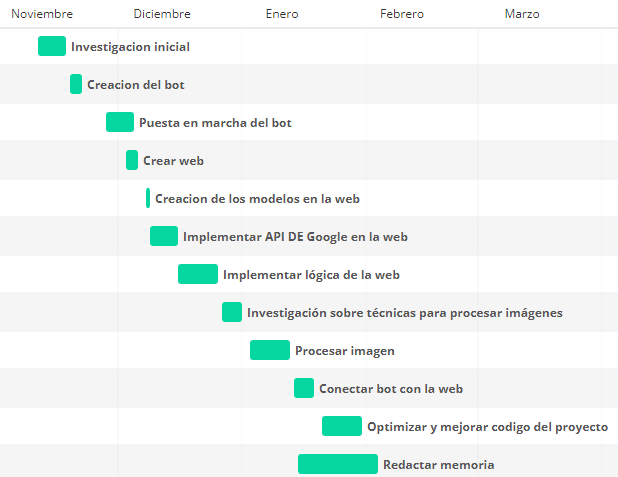
\includegraphics[scale=0.75]{imgs/gant.png}
\end{figure}
\chapter{Presupuesto}\label{int}
\thispagestyle{fancy}


\section{Desglose del presupuesto}
El coste de los recursos y gastos de personal necesarios para desarrollar la solución del sistema propuesto. Estos gastos se desglosan en dos partes: los costes de personal asociados a las tareas de dirección, diseño, programación; y el coste de los recursos necesarios o mínimos para su implantación.
\subsection{Gastos en personal}
Tomando una tasa media de 50 euros por hora, sabiendo que este proyecto tomo un tiempo dedicado al desarrollo software de alrededor de 350 horas, el precio sería de, 17500 euros, Suponiendo que haría falta un director de proyecto con una estimación de salario de 90 euros por hora sumariamos un total de 2250 euros por 25 horas de trabajo. Lo que nos deja un presupuesto de, 19750 euros para el personal.
\begin{table}[h]
\begin{center}
\begin{tabular}{| c | c | c | c | }
\hline
\multicolumn{4}{ |c| }{Gastos en personal} \\ \hline
Trabajador & Coste por horas €/h & Horas & Coste \\ \hline
Programador & 50 & 350 & 17500€ \\\hline
Director & 90 & 25 & 2250€ \\ \hline

\end{tabular}
\caption{Gasto en personal}
\label{tab:presupuesto personal}
\end{center}
\end{table}
\subsection{Gastos en software}
Las herramientas software empleadas para este proyecto tienen licencia open source, por lo tanto, no se precisa la realización de un pago para su uso.
El único pago que deberíamos de afrontar sería el despliegue de la web, el registro del dominio, así como el costo de certificado ssl.


\begin{itemize}
    \item Registro de dominio: entre 10 euros por año
    \item Hosting para la web: 150 euros por año
    \item Costo de certificado SSL: 70 euros por año
\end{itemize}

Teniendo en cuenta estos gastos nos deja un coste aproximado de 230 euros anuales

\chapter{Conclusiones}\label{int}
\thispagestyle{fancy}


\section{Resultados obtenidos}
Al acabar este proyecto, se puede concluir que este proyecto ha cumplido con los objetivos definidos inicialmente, implementación de un bot capaz de recibir imágenes y poder procesarlas, así como mandar la ubicación. Implementar una interfaz web capaz de mostrar los datos enviados por este bot.
\section{Posibles mejoras}
Teniendo en consideración la implementación del proyecto como el diseño y desarrollo base de, se presentan una serie
de mejoras de cara a un despliegue a una escala mayor o una adición de funcionalidad para
alguno de los servicios desarrollados.
\begin{enumerate}
\item Hosting en un servidor para el bot de Telegram
\item Utilizar un modelo de aprendizaje automático entrenado con imágenes etiquetadas para clasificar la imagen. Y así poder saber si la imagen subida por el usuario corresponde con la esperada.
\item En lugar de usar @csrfexempt, se debería utilizar un mecanismo de seguridad adecuado, como un token CSRF, para proteger la aplicación de ataques CSRF.
\end{enumerate}
\chapter{Valoración}\label{val}
\thispagestyle{fancy}
\section{Ética}
Este proyecto tiene dos objetivos fácilmente identificables, siendo uno el poder acercar a la ciudadanía una herramienta fácil de utilizar para poder saber la calidad del aire en cualquier lado.
Poder tener acceso a la información relativa sobre la calidad del aire fácil y accesible.

Además, el uso de tecnología para la detección de la contaminación es una forma de promover la transparencia y la responsabilidad, ya que permite a los ciudadanos y a las autoridades tener acceso a información precisa y actualizada sobre los niveles de contaminación en tiempo real.

El principio de beneficencia está presente en dar una herramienta que es capaz de otorgarnos información sobre la calidad del aire. Esta herramienta puedo ayudar a la sociedad a concienciarse sobre la calidad del aire que respiran y así poder tomar medidas preventivas para proteger su salud y la de sus seres queridos.
También puede llevar a la ciudadanía a interesarse por las fuentes de contaminación en su entorno y así poder evitarlas, así como participar en la lucha contra la contaminación del aire.


\section{Personal}
Por último, cabe señalar que el progreso del proyecto ha tenido un impacto positivo en la vida intelectual y personal de los estudiantes. En primer lugar, los conocimientos adquiridos a lo largo de los años de formación se han aplicado a los múltiples aspectos relacionados con el proyecto. El desarrollo de un bot de Telegram y el tratamiento de las imágenes, han requerido, no obstante, el aprendizaje de estos temas.
Asimismo, ha sido enriquecedor diseñar y construir una solución que pueda servir de base o punto de partida para el eventual lanzamiento del sistema a gran escala en el futuro.
\chapter{Repositorio Github }\label{Int}
\fancyhf{}% Clear header/footer
\fancyhead[L]{PROYECTO DE FIN DE GRADO}
\fancyfoot[L]{\thepage} 
El uso de Github ha sido fundamental para desarrollar de manera efectiva el proyecto, ya que me ha proporcionado un espacio donde alojar el código, con esto podía proteger este proyecto contra problemas que pudieran surgir como por ejemplo si mi ordenador quedase destruido no perdería el trabajo, ya que este está alojado en Github y podría continuar el desarrollo en otro ordenador, además permite la integración continua del código, seguido adjunto el enlace al repositorio.\\
\href{https://github.com/aitormorais/TrabajoFinGrado}{Repositorio}
\chapter{Bibliografía}\label{int}
\section{Enlaces}
\begin{enumerate}[label={[\arabic*]}]
    \item {OpenCv }\url{https://docs.opencv.org/4.x/}
    \item {Django documentación }\url{https://docs.djangoproject.com/en/4.1/}
  \item {Telegram documentación }\url{https://core.telegram.org/bots/api}
    \item {Información sobre el estado de aire a nivel estatal }\url{https://www.miteco.gob.es/es/calidad-y-evaluacion-ambiental/temas/atmosfera-y-calidad-del-aire/calidad-del-aire/documentacion-oficial/Analisis-CA.aspx}

    \item {Efectos PM2.5 y PM10 en el medio ambiente} \url{https://espanol.epa.gov/espanol/efectos-del-material-particulado-pm-sobre-la-salud-y-el-medioambiente}
    \item{Ciencia ciudadana}\url{https://ciencia-ciudadana.es/white-paper-on-citizen-science-for-europe/}
    \item{Principios de la ciencia ciudadana}\url{https://ecsa.citizen-science.net/wp-content/uploads/2021/05/ECSA_Ten_principles_of_CS_Spanish.pdf}
    \item{Anteproyecto de ley orgánica del sistema sanitario}\url{https://www.universidades.gob.es/anteproyecto-de-ley-organica-del-sistema-universitario/}
\end{enumerate}



\newpage
\thispagestyle{empty}

\thispagestyle{fancy}

\newpage
\thispagestyle{empty}
\fancypagestyle{plain}{}
\begin{appendices}
    \chapter{Anexo}\label{int}
\thispagestyle{fancy}


\section*{Anexo}
En este anexo explicaré brevemente como usar mi proyecto para medir la calidad del aire.Asi como las tecnologias usadas para llevar a cabo el proyecto de fin de grado.
\subsection{Tecnologías:}
\begin{enumerate}
    \item Django: Es un framework web de código abierto escrito en Python que permite el desarrollo rápido y eficiente de aplicaciones web.
    \item Bot en Telegram: Se utiliza para la interacción con el usuario.
    \item OpenCv: Es una librería de visión por computadora de código abierto escrita en C++ y Python, se utiliza en este proyecto para desarrollar un script capaz de detectar puntos en una imagen.
    \item Python Es un lenguaje de programación de alto nivel, interpretado y multiplataforma.
    \item SQLite: Base de datos usada para alojar la informacion relevante a la contaminación.
    \item LaTex : Para la redacción de la memoria
    \item Github: Es una forja para alojar proyectos utilizando el sistema de control de versiones Git.
\end{enumerate}
\subsection{Manual de uso :}
Lo primero que deberíamos de hacer será clonar el \hyperlink{https://github.com/aitormorais/TrabajoFinGrado}{repositorio} de GitHub con el siguiente comando:
\begin{lstlisting}[ caption=clonar repositorio ]
git clone https://github.com/aitormorais/TrabajoFinGrado
\end{lstlisting}
una vez este proceso se ha completado tendrás que instalar todas las dependencias con el siguiente comando:
 \begin{lstlisting}[ caption=instalar instalar todas las dependencias ]
pip install -r requirements.txt
\end{lstlisting} una vez las dependencias han sido instaladas será necesario tener dos terminales activas, y ejecutar en cada una de ellas el siguiente comando:
\begin{lstlisting}[ caption=arrancar web terminal 1 ]
python manage.py runserver
\end{lstlisting}
\begin{lstlisting}[ caption=arrancar bot ]
python bot.py
\end{lstlisting}

\begin{figure}[H]
\centering
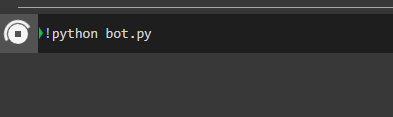
\includegraphics[scale=1]{imgs/lanzar.png}
\end{figure}

Accede a la aplicación de Telegram, es importante usarla desde el móvil, ya que por ahora no es posible mandar la ubicación desde el ordenador.Busca el siguiente nombre: 
\begin{figure}[h]
\centering

\includegraphics[scale=1]{imgs/bot.png}
\end{figure} \\
una vez estés en el bot introduce la ubicación clicando el clip y después dándole a ubicación, seguido añade la foto donde se encuentra plasmada la contaminación, acto seguido accede a la web y verás la actualización en el mapa
\begin{figure}[H]
\centering
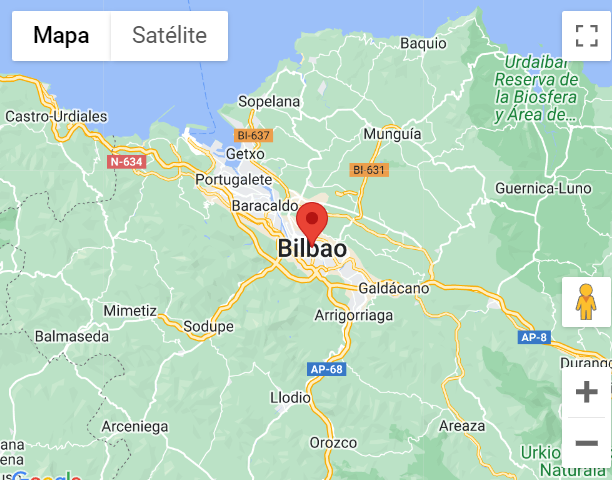
\includegraphics[scale=1]{imgs/map.png}
\end{figure}










\end{appendices}

\end{document}
